\chapter{Zanka \texttt{while}}

\section{Kaj so zanke?}

Z uporabo stavka \texttt{if} lahko torej izbrane stavke izvedemo samo v primeru, ko je nek pogoj izpolnjen. Včasih pa bi želeli izbrane stavke izvajati vse \textbf{dokler} \angl{while} je nek pogoj izpolnjen. Slednje omogočajo \textbf{zanke}. V sledečem poglavju si bomo podrobneje pogledali zanko \texttt{while}. Razliko med izvedbo pogojnega stavka \texttt{if} in zanko \texttt{while} prikazuje slika \ref{img:while_vs_if}.

\begin{figure}
    \centering
    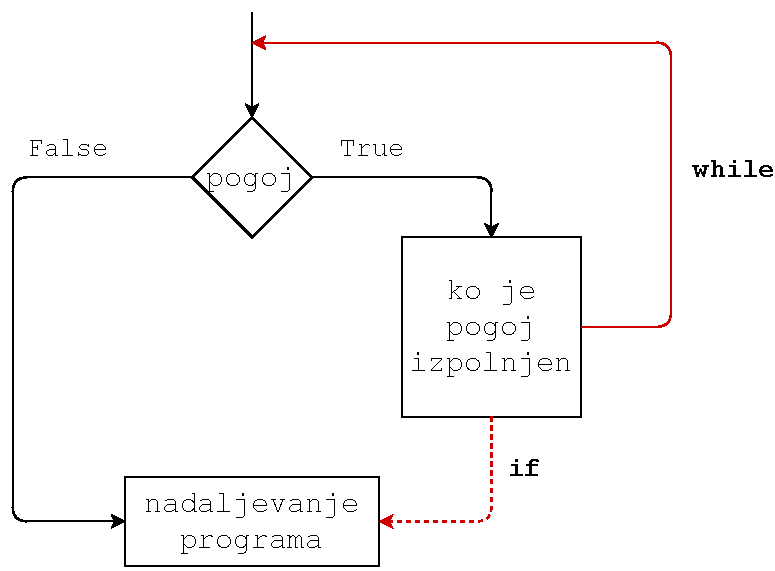
\includegraphics[width=0.5\linewidth]{img/while_vs_if.pdf}
    \caption{Razlika med izvedbo pogojnega stavka \texttt{if} (črtkana linija rdeče barve) in zanko \texttt{while} (polna linija rdeče barve). }
    \label{img:while_vs_if}
\end{figure}

\section{Zanka \texttt{while}}

Po izvedbi pogojnega dela stavka \texttt{if} se izvajanje programa nadaljuje v delu, ki sledi pogojnim stavkom. Po drugi strani se po izvedbi pogojnega dela zanke \texttt{while}, recimo tem stavkom raje \emph{telo zanke}, izpolnjenost pogoja v \emph{glavi zanke} ponovno preverja. Telo (vsebina) zanke se bo torej izvajalo vse dokler bo pogoj izpolnjen. Zanko \texttt{while} lahko zapišemo takole:
\begin{lstlisting}[language=Python]
while pogoj: # glava zanke
    # telo zanke
    ...
# nadaljevanje programa
...
\end{lstlisting}
Zapis zanke \texttt{while} je torej zelo podoben zapisu stavka \texttt{if}. Glavi zanke sledi telo zanke oziroma njena vsebina, ki se izvaja vse dokler je pogoj izpolnjen. Enemu obhodu zanke pravimo tudi \texttt{iteracija} zanke. Pogoje za izvedbo nove iteracije zanke lahko zapisujemo na popolnoma enak način kot pri stavku \texttt{if}. Prav tako kot pri stavku \texttt{if} vsebino zanke definiramo tako, da stavke znotraj telesa zanke zamikamo. Izvajanje zanke \texttt{while} ponazarja diagram poteka na sliki \ref{img:while1}.

\begin{figure}
    \centering
    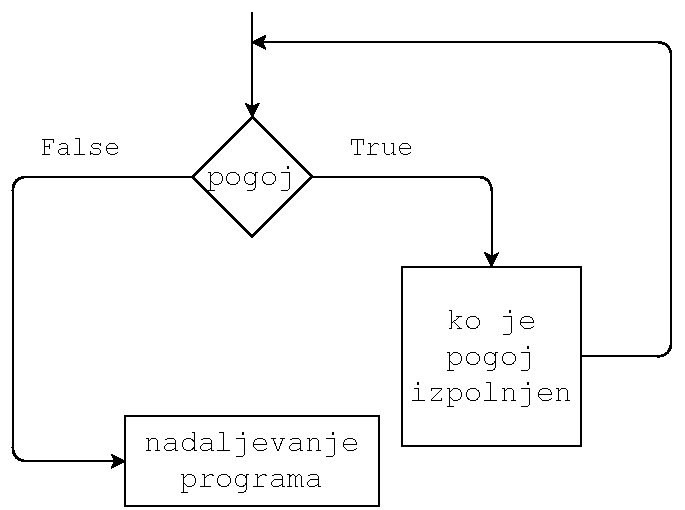
\includegraphics[width=0.5\linewidth]{img/while1.pdf}
    \caption{Potek izvajanja zanke \texttt{while}.}
    \label{img:while1}
\end{figure}

Zanke torej lahko uporabljamo takrat, ko želimo nekaj ponavljati dokler je določen pogoj izpolnjen. Npr., dokler uporabnik ne poda veljavnega vnosa, dokler ni števec dosegel določene vrednosti ali dokler sta števili različni. Končno lahko rešimo program, ki išče največji skupni delitelj dveh števil.
\begin{zgled}
Napiši program, ki od uporabnika prebere dve celi števili in poišče največji skupni delitelj teh dveh števil
\end{zgled}
\begin{resitev}
Program bo manjše število odšteval od večjega, dokler sta števili različni. Uporabili bomo torej zanko \texttt{while} (dokler sta števili različni).  Znotraj zanke bomo uporabili še stavek \texttt{if}, s pomočjo katerega bomo ugotovili, katero število je manjše. 
\begin{lstlisting}[language=Python,numbers=left]
st1 = int(input("Vnesi prvo stevilo: "))
st2 = int(input("Vnesi drugo stevilo: "))

while st1 != st2: # dokler sta stevili razlicni
    if st1 < st2: #drugo stevilo je vecje
        st2 = st2 - st1
    else: # prvo stevilo je veje
        st1 = st1 - st2

# konec vsebine zanke 
print(st1) # stevili sta tu enaki, zato je vseeno katero izpisem
\end{lstlisting}
Opomba: vsebina stavka \texttt{if} je zamaknjena dvakrat, saj je zapisana tako znotraj stavka \texttt{if} kot tudi znotraj zanke \texttt{while}!
\end{resitev}

\section{Štetje z zanko \texttt{while}}

Zanko \texttt{while} bi lahko uporabili tudi za štetje. Za ta namen je sicer boljša zanka \texttt{for}, do katere pridemo kasneje. Poglejmo si zgled.
\begin{zgled}
Napiši program, ki šteje od 0 do števila, ki ga je vnesel uporabnik. Vsa števila naj program tudi izpiše
\end{zgled}
\begin{resitev}
Število, do katerega smo prešteli, si bomo morali nekam zabeležiti, npr. v spremeneljivko z imenom \texttt{i}. Šteti bomo glede na navodila začeli s številom 0. Torej bomo spremenljivko \texttt{i} na začetku postavili na 0. Končali bomo s številom, ki ga je vnesel uporabnik, recimo \texttt{n}. Pogoj za štetje naprej bo torej \texttt{i <= n}. Znotraj zanke \texttt{while} bomo trenutno število (\texttt{i}) izpisali, poleg tega moramo pa trenutno število tudi povečati, saj bo sicer pogoj za vedno izpolnjen. 
\begin{lstlisting}[language=Python,numbers=left]
n = int(input("Vpisi stevilo do katerega zelis steti: "))
i = 0 # stevec s katerim bomo steli
while i <= n: # smo ze presteli?
    print(i)
    i = i + 1 # povecanje stevca za 1
\end{lstlisting}
\end{resitev}

\section{Stavek \texttt{+=}}
Znotraj zanke smo števec povečali za 1 z izvedbo prireditve
\begin{lstlisting}[language=Python]
i = i + 1 # povecanje stevca za 1
\end{lstlisting}
\texttt{i = i + 1}. Ker je tak način povečevanja vrednosti zelo pogost, v jeziku Python obstaja bližnjica
\begin{lstlisting}[language=Python]
i += 1 # povecanje stevca za 1
\end{lstlisting}


Kaj pa bi se zgodilo, če bi števec znotraj zanke pozabili povečati? Spremenljivka \texttt{i} oziroma števec bi ostala na vrednosti 0 tudi po izvedbi zanke, kar pomeni, da bi bil pogoj za vedno izpolnjen. Kdaj bi se taka zanka končala? Ker je pogoj vedno resničen, se taka zanka nikoli ne konča in tak program je potrebno končati na silo (v okolju Python je temu namenjena kombinacija tipk \texttt{ctrl + c}). Na take stvari moramo torej pri programiranju z zanko \texttt{while} paziti. Zanki, ki se nikoli ne konča pravimo \emph{mrtva zanka} \angl{deadlock}.

\section{Stavek \texttt{break}}

\begin{figure}
    \centering
    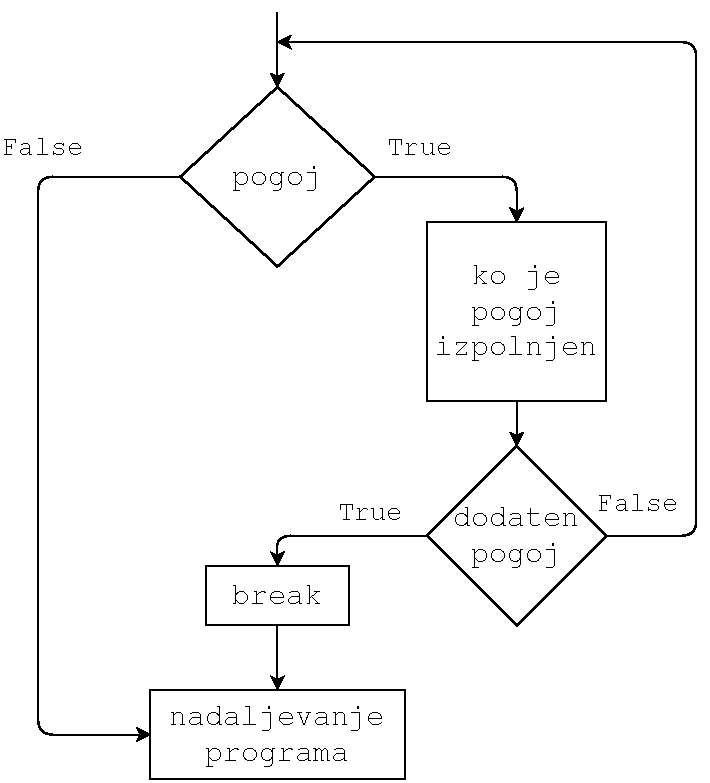
\includegraphics[width=0.5\linewidth]{img/while2.pdf}
    \caption{...}
    \label{img:while2}
\end{figure}